%
% Copyright (C) 2015-2022 The ESPResSo project
%
% This file is part of ESPResSo.
%
% ESPResSo is free software: you can redistribute it and/or modify
% it under the terms of the GNU General Public License as published by
% the Free Software Foundation, either version 3 of the License, or
% (at your option) any later version.
%
% ESPResSo is distributed in the hope that it will be useful,
% but WITHOUT ANY WARRANTY; without even the implied warranty of
% MERCHANTABILITY or FITNESS FOR A PARTICULAR PURPOSE.  See the
% GNU General Public License for more details.
%
% You should have received a copy of the GNU General Public License
% along with this program.  If not, see <http://www.gnu.org/licenses/>.
%

\documentclass[tikz]{standalone}
\begin{document}
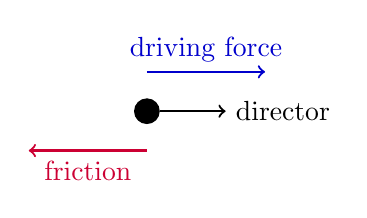
\begin{tikzpicture}[thick]
  \node[draw,fill,circle,inner sep=3pt] (A) {};
  \draw[->] (A) -- ++(1,0) node[right] {director};
  \draw[blue!80!black,->] (A) ++(0, .5) -- node[above] {driving force} ++(1.5,0);
  \draw[red!80!blue,->] (A) ++(0,-.5) -- node[below] {friction} ++(-1.5,0);
\end{tikzpicture}
\end{document}
